% Drawing 154/08-19 -- folder 154, batch 08, archive page 145 (PDF page 146).
% Transcription: grand dessin à l'encre et au crayon : un disque dont le bord porte les extrémités de sept pseudo-droites $A, B, C, D, E, F, G$ (chacune deux fois), un faisceau de fines courbes au crayon qui joignent deux points opposés du bord (un balayage), et un chemin de flèches brunes numérotées $1$ à $19$ qui passe de croisement en croisement ; les deux extrémités $E$, $D$, $C$ du côté droit sont fléchées
% Kind: disk with seven pseudo-lines, a sweep, and a path of numbered arrows. Method 2 (schematic redraw from the facsimile). Status: partial.
% Notes: Whole-page figure, redrawn as a skeleton. Drawn: the pencil rim, the two poles of the sweep (top and bottom) with five of its fine pencil curves, the seven pseudo-lines with their letters at both ends (A, B, F, G nearly straight; E nearly straight from left to right; C and D as the two curved lines that the brown arrows follow, C passing below and D above), and the brown arrows along C, D and E and from crossing to crossing in the middle, with the numbers 1 to 19 that could be read placed by their vertices. The course of C and D between their ends is read from the arrows that run along them and is not sure; the arrows of the middle (vertices 7 to 17) are approximate, several numbers are written twice on the page and only one of each is kept. Not drawn: the two wire diagrams at the bottom right (the transcription describes them in the same note), the hatched crescents, and the small sketches of lines at the upper right. Redrawn 2026-11-12 (issue 128): to check again.
% Coordinates: 1 unit = 1 mm = 1/100 of the crop width (bbox in page fractions: [0.26, 0.095, 0.8, 0.49]).
% Redrawn by Claude (claude-fable-5-2), issue #128, 2026-11-12; not checked by a human; not compiled (no TeX in the session).
% Rights: reproduces part of the work -- behind RENDER_TRANSCRIPTS, never published by itself.
\documentclass[tikz,border=3pt]{standalone}
\usepackage{amsmath,amssymb}
\usetikzlibrary{patterns,arrows.meta}
\tikzset{Br/.style={brown!80!black}, pencil/.style={black!45}, struck/.style={black!35}, mpt/.style={circle,draw,inner sep=1.3pt}, pt/.style={circle,fill,inner sep=0.9pt}, opt/.style={circle,draw,fill=white,inner sep=1.1pt}}
\begin{document}
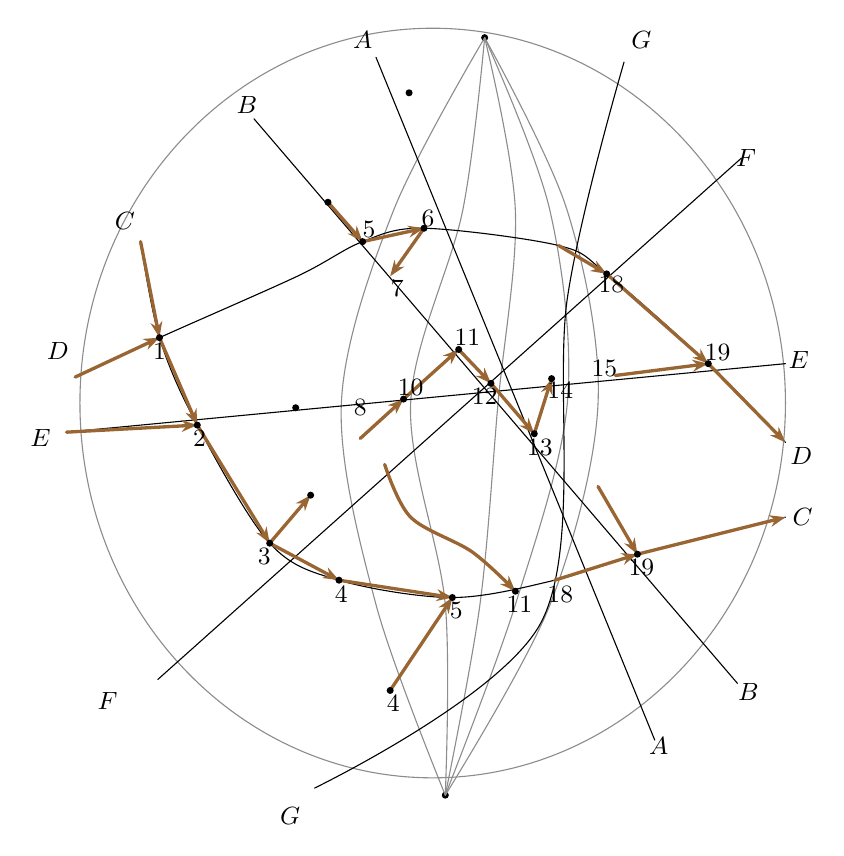
\begin{tikzpicture}[x=1mm,y=1mm,line cap=round,line join=round,font=\scriptsize]
\draw[pencil] (51,-48.6) ellipse[x radius=44.8, y radius=47.6];
\node[pt] at (57.6,-2.2) {};
\node[pt] at (52.6,-98.4) {};
\draw[pencil] plot[smooth, tension=0.55] coordinates {(57.6,-2.2) (46,-24.2) (39.4,-48.6) (43.8,-74.2) (52.6,-98.4)};
\draw[pencil] plot[smooth, tension=0.55] coordinates {(57.6,-2.2) (54.8,-24.2) (48.2,-48.6) (52.6,-74.2) (52.6,-98.4)};
\draw[pencil] plot[smooth, tension=0.55] coordinates {(57.6,-2.2) (61.5,-24.2) (59.3,-48.6) (57,-74.2) (52.6,-98.4)};
\draw[pencil] plot[smooth, tension=0.55] coordinates {(57.6,-2.2) (65.9,-24.2) (68.1,-48.6) (61.5,-74.2) (52.6,-98.4)};
\draw[pencil] plot[smooth, tension=0.55] coordinates {(57.6,-2.2) (68.1,-24.2) (72,-48.6) (65.9,-74.2) (52.6,-98.4)};
\draw (43.8,-4.7) -- (79.2,-91.4);
\draw (28.3,-12.5) -- (89.7,-84.2);
\draw (16.1,-83.7) -- (90.2,-17.5);
\draw plot[smooth, tension=0.55] coordinates {(75.3,-5.3) (68.1,-35.3) (64.8,-76.4) (36,-97.5)};
\draw (4.5,-52.3) -- (95.8,-43.6);
\draw plot[smooth, tension=0.55] coordinates {(13.9,-28.1) (16.3,-40.3) (21.1,-51.4) (30.3,-66.4) (39.1,-71.1) (53.5,-73.3) (66.5,-71.1) (77,-67.8) (95.8,-63.1)};
\draw plot[smooth, tension=0.55] coordinates {(5.6,-45.3) (16.3,-40.3) (33.8,-32.5) (42.1,-28.1) (49.9,-26.4) (67,-28.6) (73.1,-32.2) (86,-43.6) (95.8,-53.6)};
\draw[Br,very thick,-{Stealth[length=2mm]}] (13.9,-28.1) -- (16.3,-40.3);
\draw[Br,very thick,-{Stealth[length=2mm]}] (16.3,-40.3) -- (21.1,-51.4);
\draw[Br,very thick,-{Stealth[length=2mm]}] (21.1,-51.4) -- (30.3,-66.4);
\draw[Br,very thick,-{Stealth[length=2mm]}] (30.3,-66.4) -- (39.1,-71.1);
\draw[Br,very thick,-{Stealth[length=2mm]}] (39.1,-71.1) -- (53.5,-73.3);
\draw[Br,very thick,-{Stealth[length=2mm]}] (5.6,-45.3) -- (16.3,-40.3);
\draw[Br,very thick,-{Stealth[length=2mm]}] (4.5,-52.3) -- (21.1,-51.4);
\draw[Br,very thick,-{Stealth[length=2mm]}] (45.6,-85.1) -- (53.5,-73.3);
\draw[Br,very thick,-{Stealth[length=2mm]}] (30.3,-66.4) -- (35.5,-60.3);
\draw[Br,very thick,-{Stealth[length=2mm]}] (37.7,-23.1) -- (42.1,-28.1);
\draw[Br,very thick,-{Stealth[length=2mm]}] (42.1,-28.1) -- (49.9,-26.4);
\draw[Br,very thick,-{Stealth[length=2mm]}] (49.9,-26.4) -- (45.6,-32.5);
\draw[Br,very thick,-{Stealth[length=2mm]}] (41.8,-53.1) -- (47.3,-48.1);
\draw[Br,very thick,-{Stealth[length=2mm]}] (47.3,-48.1) -- (54.3,-41.8);
\draw[Br,very thick,-{Stealth[length=2mm]}] (54.3,-41.8) -- (58.4,-46.1);
\draw[Br,very thick,-{Stealth[length=2mm]}] (58.4,-46.1) -- (63.9,-52.5);
\draw[Br,very thick,-{Stealth[length=2mm]}] (63.9,-52.5) -- (66.1,-45.5);
\draw[Br,very thick,-{Stealth[length=2mm]}] plot[smooth, tension=0.55] coordinates {(44.9,-56.4) (48.2,-63.1) (56,-67.5) (61.5,-72.5)};
\draw[Br,very thick,-{Stealth[length=2mm]}] (67,-28.6) -- (73.1,-32.2);
\draw[Br,very thick,-{Stealth[length=2mm]}] (73.1,-32.2) -- (86,-43.6);
\draw[Br,very thick,-{Stealth[length=2mm]}] (86,-43.6) -- (95.8,-53.6);
\draw[Br,very thick,-{Stealth[length=2mm]}] (74.2,-45.1) -- (86,-43.6);
\draw[Br,very thick,-{Stealth[length=2mm]}] (66.5,-71.1) -- (77,-67.8);
\draw[Br,very thick,-{Stealth[length=2mm]}] (77,-67.8) -- (95.8,-63.1);
\draw[Br,very thick,-{Stealth[length=2mm]}] (72,-59.2) -- (77,-67.8);
\node[pt] at (16.3,-40.3) {};
\node[pt] at (21.1,-51.4) {};
\node[pt] at (30.3,-66.4) {};
\node[pt] at (39.1,-71.1) {};
\node[pt] at (53.5,-73.3) {};
\node[pt] at (45.6,-85.1) {};
\node[pt] at (35.5,-60.3) {};
\node[pt] at (42.1,-28.1) {};
\node[pt] at (49.9,-26.4) {};
\node[pt] at (47.3,-48.1) {};
\node[pt] at (54.3,-41.8) {};
\node[pt] at (58.4,-46.1) {};
\node[pt] at (63.9,-52.5) {};
\node[pt] at (66.1,-45.5) {};
\node[pt] at (73.1,-32.2) {};
\node[pt] at (86,-43.6) {};
\node[pt] at (77,-67.8) {};
\node[pt] at (61.5,-72.5) {};
\node[pt] at (48,-9.2) {};
\node[pt] at (37.7,-23.1) {};
\node[pt] at (33.6,-49.2) {};
\node[inner sep=1pt] at (42.1,-2.5) {\small $A$};
\node[inner sep=1pt] at (79.7,-92.2) {\small $A$};
\node[inner sep=1pt] at (27.4,-10.8) {\small $B$};
\node[inner sep=1pt] at (91.1,-85.3) {\small $B$};
\node[inner sep=1pt] at (11.9,-25.5) {\small $C$};
\node[inner sep=1pt] at (98,-63.1) {\small $C$};
\node[inner sep=1pt] at (3.4,-42) {\small $D$};
\node[inner sep=1pt] at (97.8,-55.3) {\small $D$};
\node[inner sep=1pt] at (1.2,-53.1) {\small $E$};
\node[inner sep=1pt] at (97.5,-43.1) {\small $E$};
\node[inner sep=1pt] at (9.7,-86.4) {\small $F$};
\node[inner sep=1pt] at (90.8,-17.5) {\small $F$};
\node[inner sep=1pt] at (77.5,-2.5) {\small $G$};
\node[inner sep=1pt] at (32.9,-101.1) {\small $G$};
\node[inner sep=1pt] at (16.3,-42) {\small 1};
\node[inner sep=1pt] at (21.4,-53.1) {\small 2};
\node[inner sep=1pt] at (29.6,-68.1) {\small 3};
\node[inner sep=1pt] at (39.4,-72.9) {\small 4};
\node[inner sep=1pt] at (54,-75) {\small 5};
\node[inner sep=1pt] at (46,-86.7) {\small 4};
\node[inner sep=1pt] at (42.9,-26.6) {\small 5};
\node[inner sep=1pt] at (50.4,-25.1) {\small 6};
\node[inner sep=1pt] at (46.5,-34) {\small 7};
\node[inner sep=1pt] at (41.8,-49.2) {\small 8};
\node[inner sep=1pt] at (48.2,-46.6) {\small 10};
\node[inner sep=1pt] at (55.4,-40.3) {\small 11};
\node[inner sep=1pt] at (57.6,-47.8) {\small 12};
\node[inner sep=1pt] at (64.6,-54.2) {\small 13};
\node[inner sep=1pt] at (67.2,-47) {\small 14};
\node[inner sep=1pt] at (72.8,-44.2) {\small 15};
\node[inner sep=1pt] at (73.7,-33.6) {\small 18};
\node[inner sep=1pt] at (87.2,-42.2) {\small 19};
\node[inner sep=1pt] at (62,-74.2) {\small 11};
\node[inner sep=1pt] at (67.2,-72.9) {\small 18};
\node[inner sep=1pt] at (77.5,-69.5) {\small 19};
\end{tikzpicture}
\end{document}
